\title{Engineering inclusivity in online conversations: early results and how to proceed}
\author{Alberto Cottica}
\date{August 2016}

\documentclass{article}
\usepackage{graphicx}
\usepackage{subcaption}
\usepackage{mathtools}
\usepackage{csquotes}
\graphicspath{ {./Paper3Images/} {./Paper3Images/First_simulations/}  }
\usepackage{hyperref}
\usepackage{enumitem}
\usepackage{subcaption} 

\setlength{\parindent}{0em}
\setlength{\parskip}{1em}

\begin{document}

\maketitle

\tableofcontents

\section{Stress-testing the Kim model}

I spent some time verifying the robustness of the model in \cite{kim2015group}. I removed three assumptions from it:

\begin{enumerate}
	\item  The community no longer starts with a substantial group of founders, all having positive intimacy with each other.
	\item Online community members no longer always engage in interaction at each time period. They now have to make a choice on whether to engage in communication at each time period. Their probability of doing so increases with the communications received in the previous period.
	\item Members no longer leave the community if their membership strength falls below a certain level.
\end{enumerate}

Removing the first assumption lends more generality to the model. Removing the other two makes the model more realistic on one hand, but introduces a fresh problem: community members, even if ignored by others, will continue to engage in communication forever (although with a probability at each period lower than that of members who do receive communications). 

The main result of \cite{kim2015group} seems to be robust to the removal of these assumptions. In all simulations I have run I was able to introduce significant inequality on the distribution of membership strength by increasing the intimacy parameter. 

\begin{figure}
  \begin{subfigure}[b]{0.5\textwidth}
    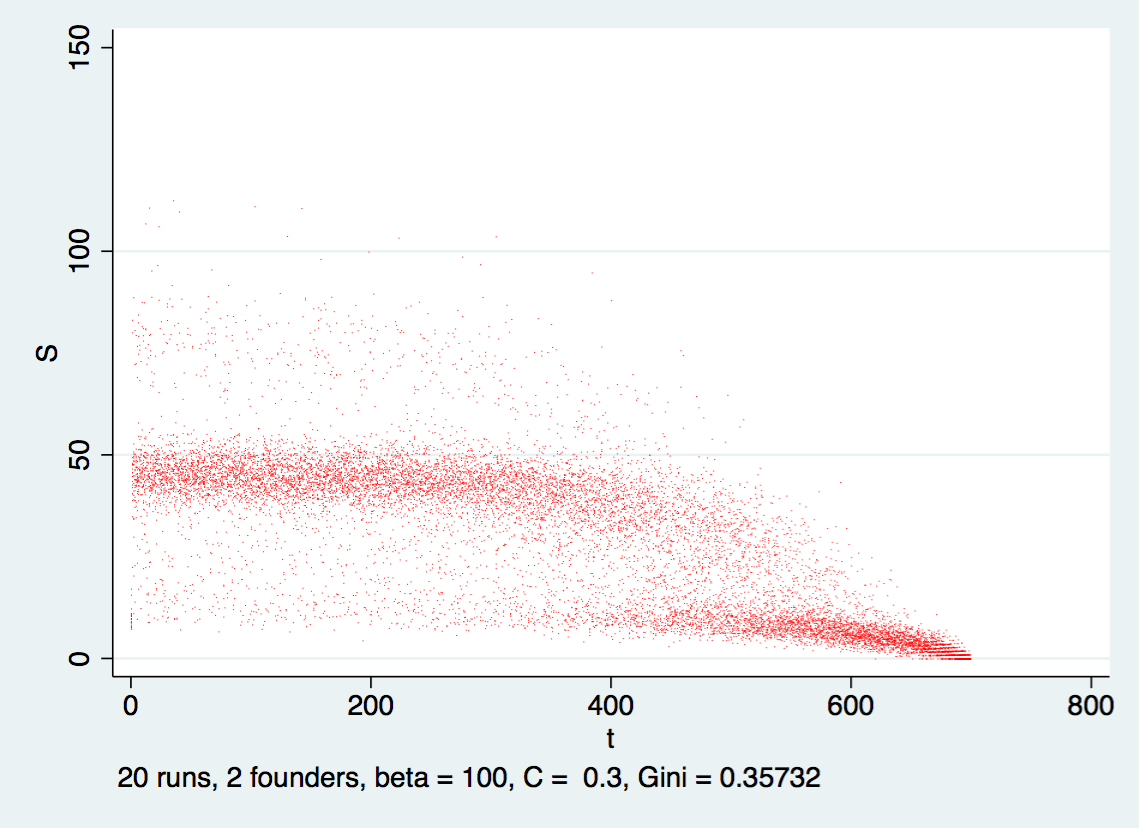
\includegraphics[width=\textwidth]{HighIntimacy2.png}
    \caption{With high intimacy strength}
    \label{highIntimacy}
  \end{subfigure}
  %
  \begin{subfigure}[b]{0.5\textwidth}
    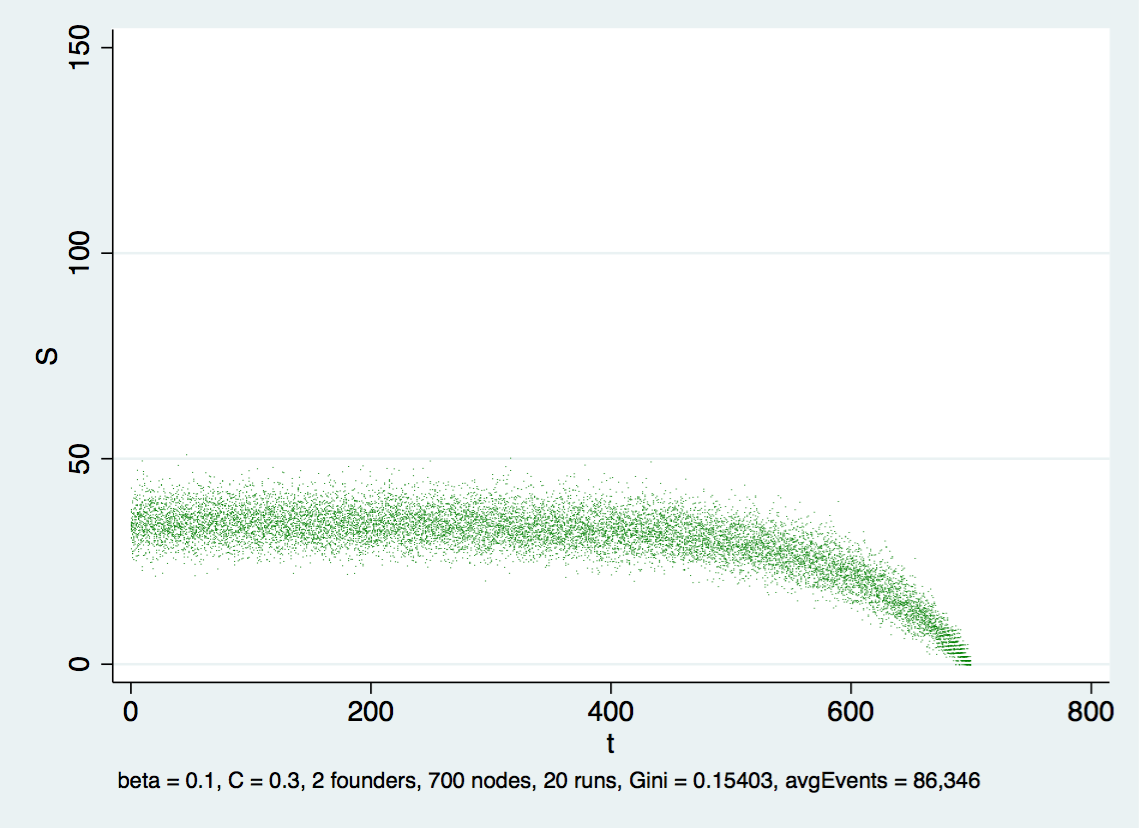
\includegraphics[width=\textwidth]{LowIntimacy.png}
    \caption{With low intimacy strength}
    \label{lowIntimacy}
  \end{subfigure}
  \caption{Distribution of membership strength as the intimacy strength parameter varies.}
\end{figure}

The distribution becomes more inequal if:

\begin{itemize}
	\item The simulation starts with a relatively large number of  "founders", all connected to each other by nonzero intimacy values (assumption 1 above is upheld).
	\item The average number of communication events per community member and per time period increases (community members are "chattier"). 
	\item The marginal probability of engaging in communication with respect to having received a communication in the previous period increases (community members are "more responsive").
	\item Node removal is possible (assumption 3 above is upheld).
\end{itemize}

\section{Model objectives}

We can think of \cite{kim2015group} as a polar model, in which the conditions are tilted in favour of high inequality of membership. In the more general world of this paper, we would like to consider the situation of an organization that is running an online community. It has four goals.

\begin{enumerate}
	\item \textit{Output}: the number of communication events that take place therein in a given time interval.
	\item  \textit{Diversity}: the inequality of the distribution between the number of communication events initiated by members. 
	\item \textit{Social capital}: the sum total of the membership strength of each individual member.
	\item \textit{Inclusivity}: the inequality of the distribution of membership strength across the community.
\end{enumerate}

These goals are pursued by means of \textit{policies}, enacted by one special agent, the online community manager. We consider two policies widely present in real-world online communities:
\begin{itemize}
	\item \textit{Onboarding}, aimed at positive reinforcement to the act of joining the community. The community manager initiates exactly one communication (a welcome message) with each member, in the time period in which the latter joins the community.
	\item \textit{Engagement}, aimed at positive reinforcement to the act of initiating communications. The community manager initiates exactly one communication (a comment) with each member who has herself initiated communication with anyone in the period before the current one.
\end{itemize}  

The model aims to explore the hypothesis that onboarding and engagement policies have spread because they produce more active, high social capital, diverse, inclusive online communities. To do this, we:

\begin{itemize}
	\item Characterize four policy scenarios: no policy (baseline); onboarding, but no engagement; engagement, but no onboarding; both onboarding and engagement.
	\item Establish indicators for the four organizational goals stated above. Output can be measured in number of contributions; social capital in overall membership strength. Inequalities can be measured in various ways: provisionally I am starting with the Gini coefficient.
	\item For each policy scenario, run a high number of simulations corresponding to a vector of the key parameters.
	\item Test the hypothesis that the indicator values in each of the three non-baseline policy scenarios are identical to those in the baseline. 
\end{itemize}

An interesting side effect of this approach is to explore potential tradeoffs across policy objectives. For example, more active communities could turn out to be less inclusive. 

\section{Where shall we take the paper?}

The model introduced in \cite{kim2015group} turned out to be rich in both insight and complexities. The parameter space is potentially high-dimensional, and the computational load is substantial. It is very possible to get lost. In what follows, I ask some questions and propose a way forward.

\subsection{Model core: the policies}

I propose that the paper zeroes in on policies for online community management and their effect. This is what strings together the whole thesis. In practice, this means:

\begin{enumerate}
	\item Asserting that the model in \cite{kim2015group} is a fairly general description of social forces at work in real-world online communities.
	\item Describing the model, and the adds-on that cover policies.
	\item Running simulations of 8 scenarios. Two of them are baselines (one with low intimacy strength, the other with high intimacy strength); the remaining six cover the three policy scenarios with low -and the three with high intimacy strength.
	\item Running the statistical tests described above and discussing their results. 
\end{enumerate}

This gives a first answer to the question: do the policies contribute towards our organizational goals \textit{in the model}? If so, is it possible that community management practices \textit{in the real world} have evolved because of this contribution?

Everything else goes in one or more appendixes.  

\begin{figure}
	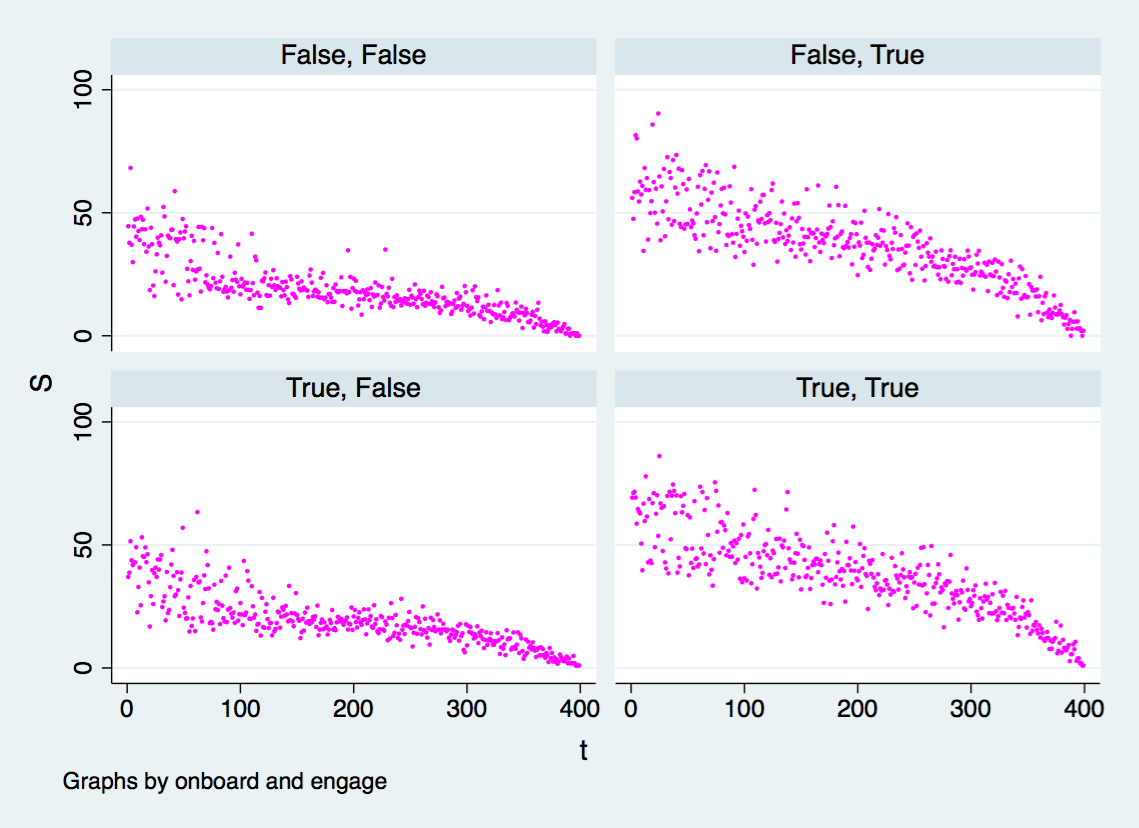
\includegraphics[width = \textwidth]{no_node_removal.png} 
	\caption{The basic model with high intimacy strength under the four possible policy scenarios. Only one run of the model has been computed.}
	\label{fig:noNodeRemoval}
\end{figure}

\subsection{Stress-testing the Kim model (redux)}

I ran several simulations to debunk what really drives the model in \cite{kim2015group}. It turns out that some assumptions that are not really discussed in the paper have a strong effect: for example, assuming one communication event per user per time period (unrealistically high) enhances the effect of intimacy strength, leading to a higher inequality of membership strength. The same can be said of the possibility of node removal. Despite this, the main result seems to be robust: you can always "break" equality in membership strength distribution by jacking up the value of the intimacy strength parameter. Other results do not necessarily carry through, like "there is a phase transition around a value of the intimacy strength parameter $\beta$ equal to 3.5".

An appendix could be dedicated to discussing this. Policy is not especially relevant for this part of the paper. We need to run simulations on the cases of low vs. high chattiness; of node removal vs. no node removal; and large clique of founders vs. small clique of founders. As before, we need two baselines, one with low - and the other with high intimacy strength. It runs to another 6 simulations (given that the baseline is the same as that in the main text of the paper). 

\begin{figure}
	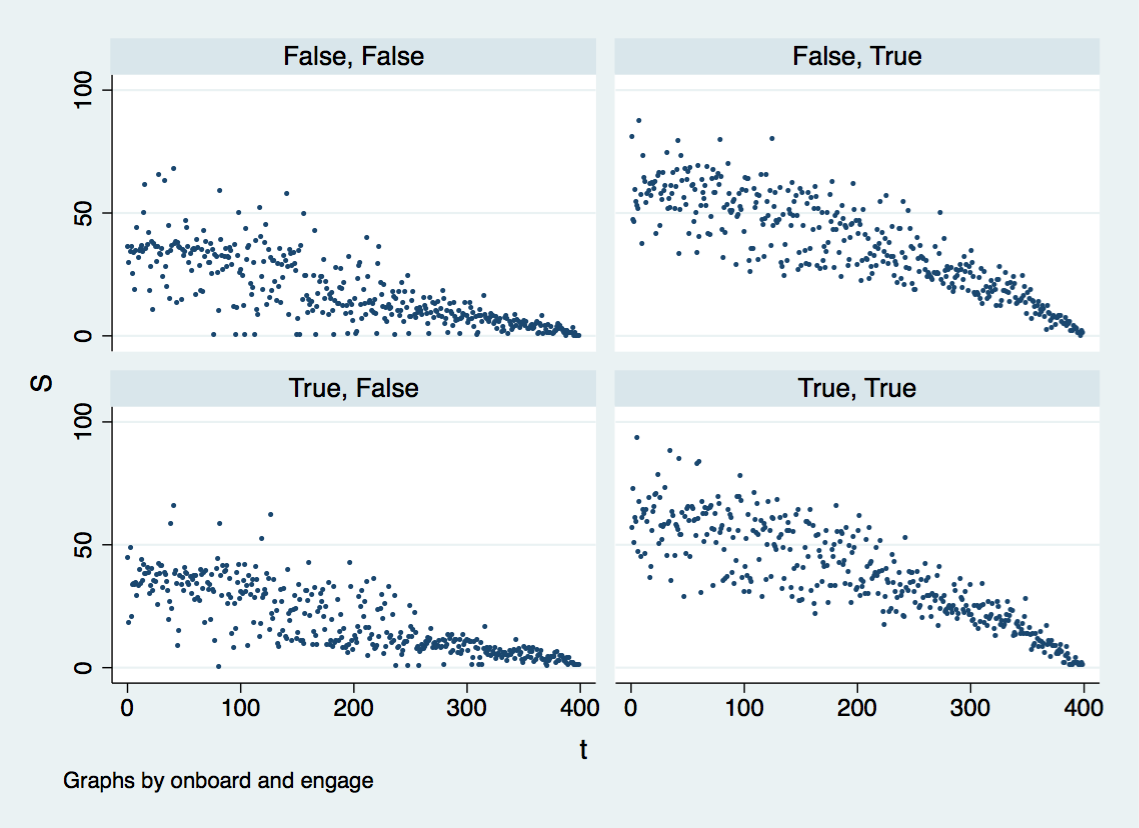
\includegraphics[width = \textwidth]{node_removal.png} 
	\caption{The basic model with high intimacy strength under the four possible policy scenarios, with node removal. Compare with figure \ref{fig:noNodeRemoval}. Only one run of the model has been computed.}
	\label{fig:nodeRemoval}
\end{figure}

\subsection{Exploring parameter space}

We could then dedicate a further section of the paper to what happens to policy effectiveness under different specifications. Of course, the organization cannot choose the state of the world: people are more or less chatty, and they decide to remove themselves from the community or not. But we could discuss how the policies become more or less effective according to the state of the world. This would mean more simulations and more discussions, of course.

\subsection{Computational load}

Running these models takes up substantial computing time. So far I have been limiting myself to batches of 20 runs each with the same parameters. Over four policy cases, that easily runs to 24 hours. Batches of 100 runs per value of the same parameter vector is probably not practical with my home machine. When Guy comes back from holiday I will ask for his help. 

\subsection{Questions}

\begin{enumerate}
	\item Do you agree with dividing the content between core (in the main text) and appendixes? 
	\item Do you think it makes sense to have an appendix dedicated to exploring and stress-testing the Kim model?
	\item Do you think it makes sense to have an appendix dedicated to exploring the parameter space?
	\item How should I measure distribution inequality for this particular problem?
	\item What is the minimum number of runs per batch that I can get away with?
\end{enumerate}

\bibliographystyle{plain}
\bibliography{Engineering_inclusivity}
	
\end{document}